\documentclass[11pt, a4paper]{article}
\usepackage{pdfpages}
\usepackage{parallel}
\usepackage[T2A]{fontenc}
%\usepackage{ucs}
\usepackage[utf8]{inputenc}
\usepackage[english,russian]{babel}
\usepackage{hyperref}
\usepackage{rotating}
\usepackage[inner=2cm,top=1.8cm,outer=2cm,bottom=2.3cm,nohead]{geometry}
%\usepackage{listings}
\usepackage{graphicx}
\usepackage{wrapfig}
\usepackage{longtable}
\usepackage{indentfirst}
\usepackage{array}
\usepackage{tikzsymbols}
\usepackage{soul}
\usepackage[ruled,vlined]{algorithm2e}
\usepackage{qrcode}
\counterwithout{figure}{section} 

\usepackage{url}
\makeatletter
\g@addto@macro{\UrlBreaks}{\UrlOrds}
\makeatother

\newcolumntype{P}[1]{>{\raggedright\arraybackslash}p{#1}}
\frenchspacing
%\usepackage{fixltx2e} %text sub- and superscripts
\usepackage{icomma} % коскі ў матэматычным рэжыме
%\PreloadUnicodePage{4}

\newcommand{\longpage}{\enlargethispage{\baselineskip}}
\newcommand{\shortpage}{\enlargethispage{-\baselineskip}}

\def\switchlang#1{\expandafter\csname switchlang#1\endcsname}
\def\switchlangbe{
\let\saverefname=\refname%
\def\refname{Літаратура}%
\def\figurename{Іл.}%
}
\def\switchlangru{
\let\saverefname=\refname%
\let\savefigurename=\figurename%
\def\refname{Литература}%
\def\figurename{Рис.}%
}
\def\switchlangen{
\let\saverefname=\refname%
\def\refname{References}%
\def\figurename{Fig.}%
}

\hyphenation{admi-ni-stra-tive}
\hyphenation{ex-pe-ri-ence}
\hyphenation{fle-xi-bi-li-ty}
\hyphenation{Py-thon}
\hyphenation{ma-the-ma-ti-cal}
\hyphenation{re-ported}
\hyphenation{imp-le-menta-tions}
\hyphenation{pro-vides}
\hyphenation{en-gi-neering}
\hyphenation{com-pa-ti-bi-li-ty}
\hyphenation{im-pos-sible}
\hyphenation{desk-top}
\hyphenation{elec-tro-nic}
\hyphenation{com-pa-ny}
\hyphenation{de-ve-lop-ment}
\hyphenation{de-ve-loping}
\hyphenation{de-ve-lop}
\hyphenation{da-ta-ba-se}
\hyphenation{plat-forms}
\hyphenation{or-ga-ni-za-tion}
\hyphenation{pro-gramming}
\hyphenation{in-stru-ments}
\hyphenation{Li-nux}
\hyphenation{sour-ce}
\hyphenation{en-vi-ron-ment}
\hyphenation{Te-le-pathy}
\hyphenation{Li-nux-ov-ka}
\hyphenation{Open-BSD}
\hyphenation{Free-BSD}
\hyphenation{men-ti-on-ed}
\hyphenation{app-li-ca-tion}

\def\progref!#1!{\texttt{#1}}
\renewcommand{\arraystretch}{2} %Іначай формулы ў матрыцы зліпаюцца з лініямі
\usepackage{array}

\def\interview #1 (#2), #3, #4, #5\par{

\section[#1, #3, #4]{#1 -- #3, #4}
\def\qname{LVEE}
\def\aname{#1}
\def\q ##1\par{{\noindent \bf \qname: ##1 }\par}
\def\a{{\noindent \bf \aname: } \def\qname{L}\def\aname{#2}}
}

\def\interview* #1 (#2), #3, #4, #5\par{

\section*{#1\\{\small\rm #3, #4. #5}}
\ifx\ParallelWhichBox\undefined%
    \addcontentsline{toc}{section}{#1, #3, #4}%
\else%
\ifnum\ParallelWhichBox=0%
    \addcontentsline{toc}{section}{#1, #3, #4}%
\fi\fi%

\def\qname{LVEE}
\def\aname{#1}
\def\q ##1\par{{\noindent \bf \qname: ##1 }\par}
\def\a{{\noindent \bf \aname: } \def\qname{L}\def\aname{#2}}
}

\newcommand{\interviewfooter}[1]{
\vskip 1em
\noindent \textit{#1}
}

\AtEndDocument{\vfill\centering \qrcode{https://github.com/fiowro/mouses/blob/main/\jobname.pdf}}

\switchlang{ru}
\begin{document}

\title{1984 "--- Mindset Mouse}
\date{}
\maketitle
\selectlanguage{russian}

Mindset Mouse "--- это мышь, которая шла в комплекте с персональным компьютером Mindset. Компьютер Mindset был выпущен в 1984 году компанией Mindset Corporation, и находился в продаже всего год. В техническом плане он был частично совместим с IBM PC, оснащался процессором Intel 80186 и нестандартной графической подсистемой, обладавшей повышенными возможностями, включая аппаратное ускорение некоторых типовых графических операций \cite{byteMagazine}.

Реальным производителем мыши выступила японская компания Alps "--- производитель первой японской мыши, Sharp MZ-1X10, представленной на японском рынке годом ранее.

\begin{figure}[h]
   \centering
    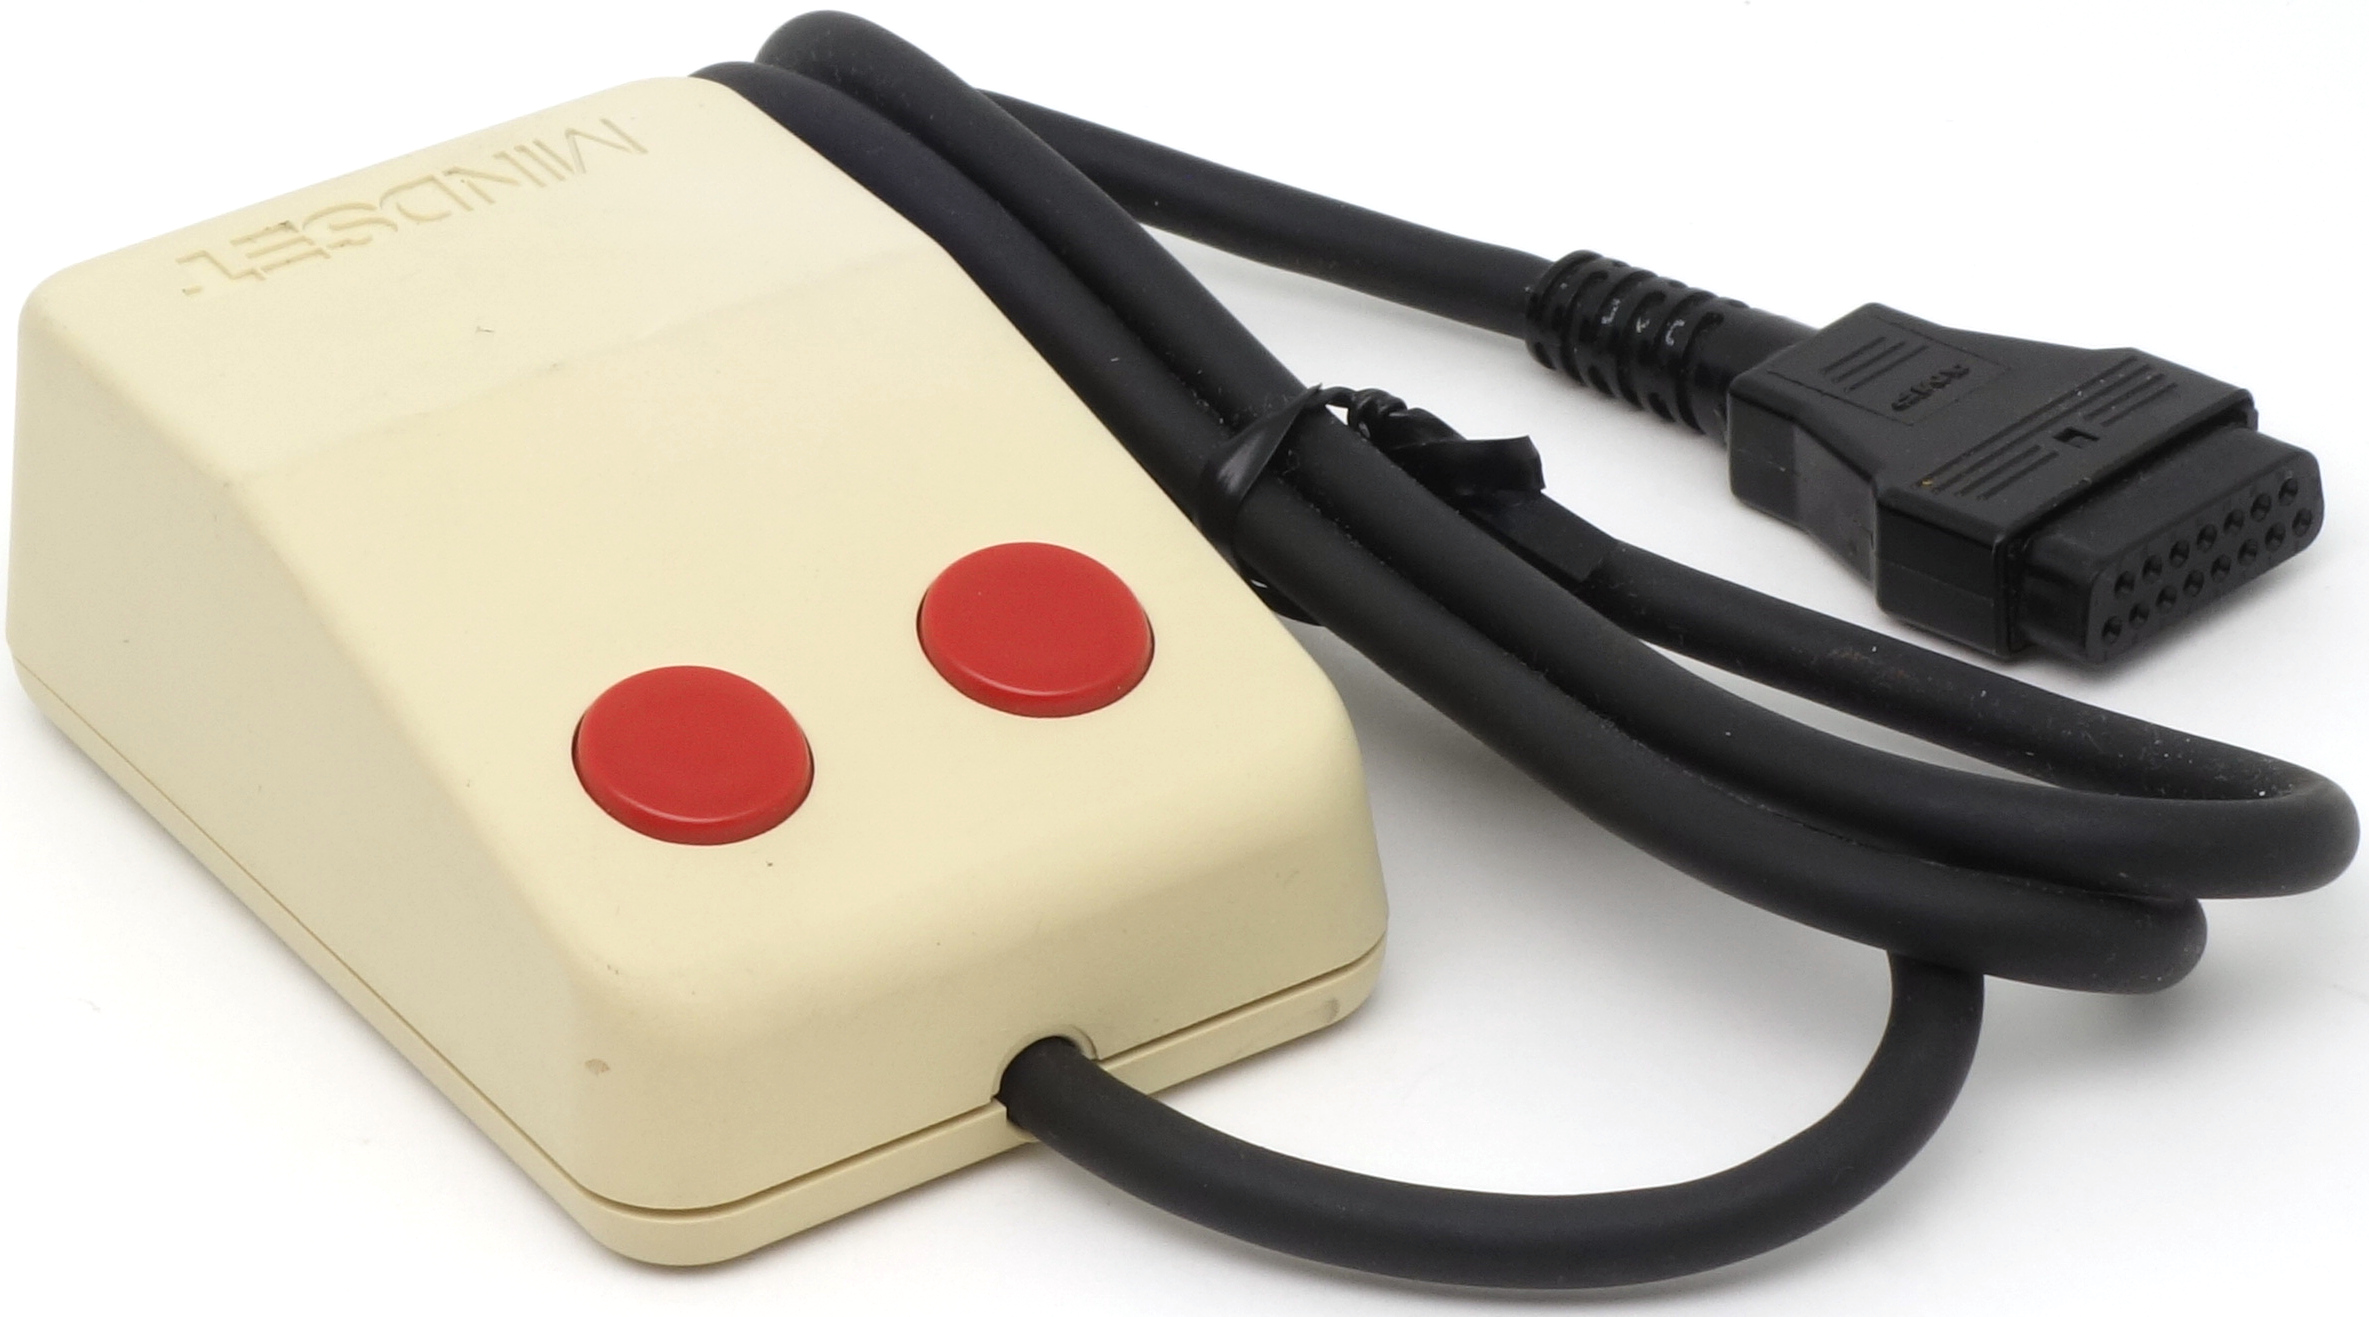
\includegraphics[scale=0.6]{1984_mindset_mouse/pic_30.jpg}
    \caption{Mindset Mouse}
    \label{fig:MindsetMousePic}
\end{figure}

В конструктивном плане мышь Mindset и MZ-1X10 имеют чрезвычайно много общего. Корпус мыши представляет собой бежевый параллелепипед со слегка скругленными гранями и клиновидным срезом верхней части корпуса, на котором расположена пара круглых красных кнопок (рис. \ref{fig:MindsetMousePic}). Благодаря этим необычным контрастным кнопкам Mindset Mouse имеет запоминающийся вид и потому постоянно присутствует в рекламных материалах компьютеров Mindset \cite{adv}.

\begin{figure}[h]
    \centering
    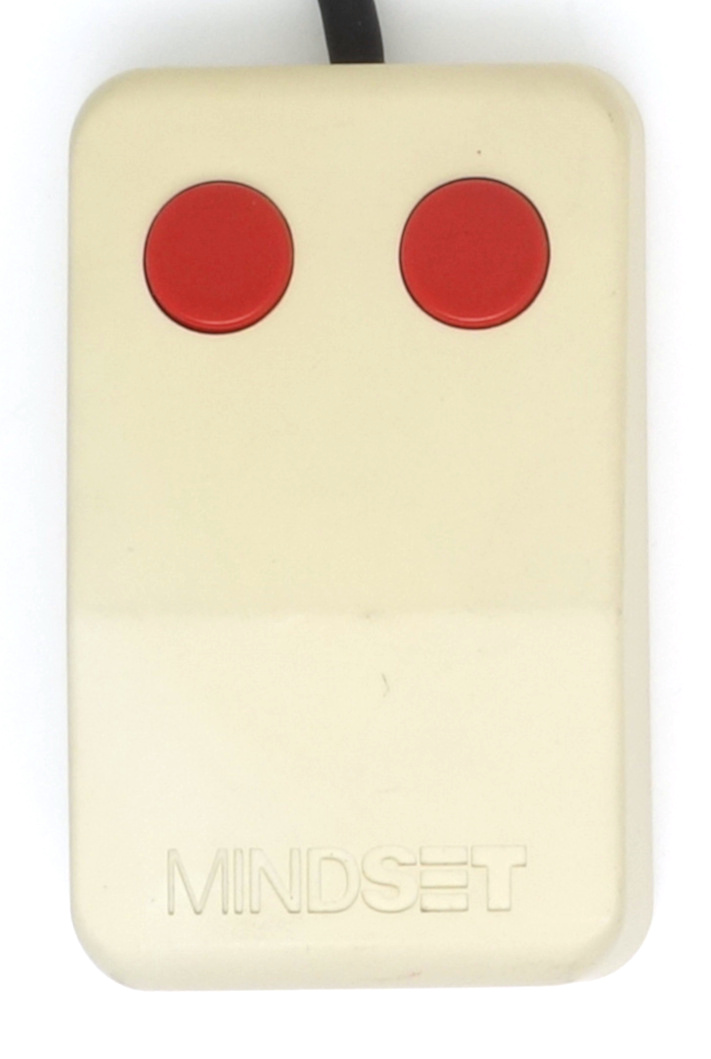
\includegraphics[scale=0.55]{1984_mindset_mouse/top_30.jpg}
    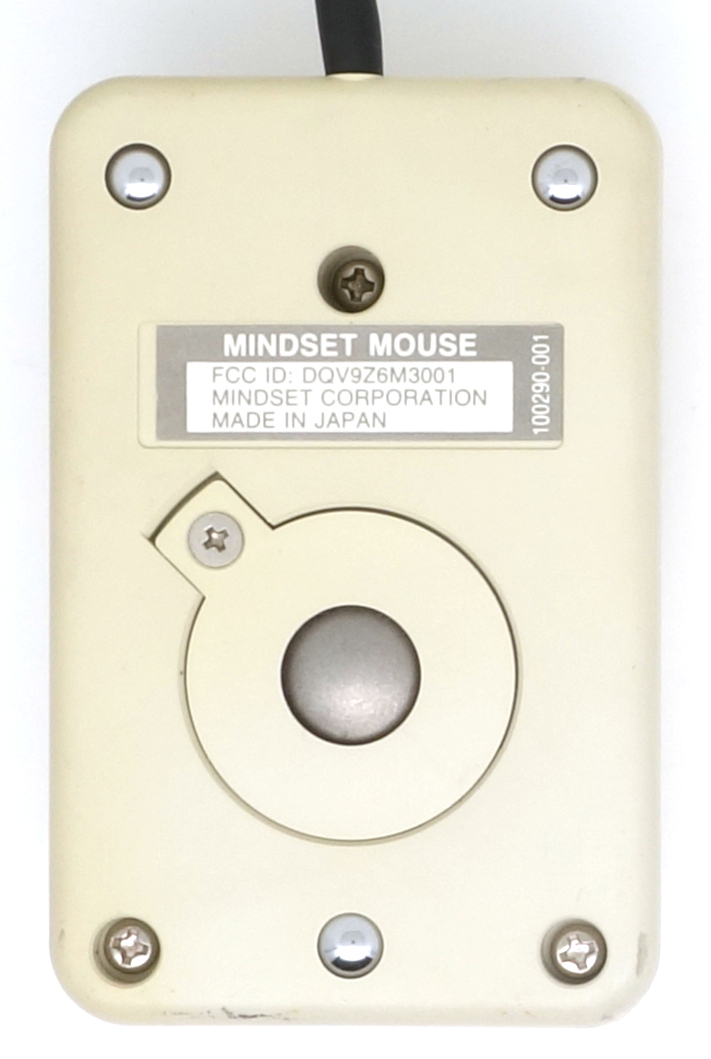
\includegraphics[scale=0.55]{1984_mindset_mouse/bottom_30.jpg}
    \caption{Mindset Mouse, вид сверху и снизу}
    \label{fig:MindsetMouseTopAndBottom}
\end{figure}

Нижняя сторона мыши аналогична модели MZ-1X10: она демонстрирует стальной шар, три металлических шарика, облегчающие скольжение мыши, и съёмное кольцо, позволяющее извлечь шар для чистки. Вариант кольца на защелках еще не был придуман, поэтому его требуется отвинчивать с помощью отвертки. Пластиковый ограничитель, защищающий провод от повреждения в месте его выхода из корпуса мыши, конструкцией не предусмотрен (рис. \ref{fig:SharpMZ1x10TopAndBottom}).

\begin{figure}[h]
    \centering
    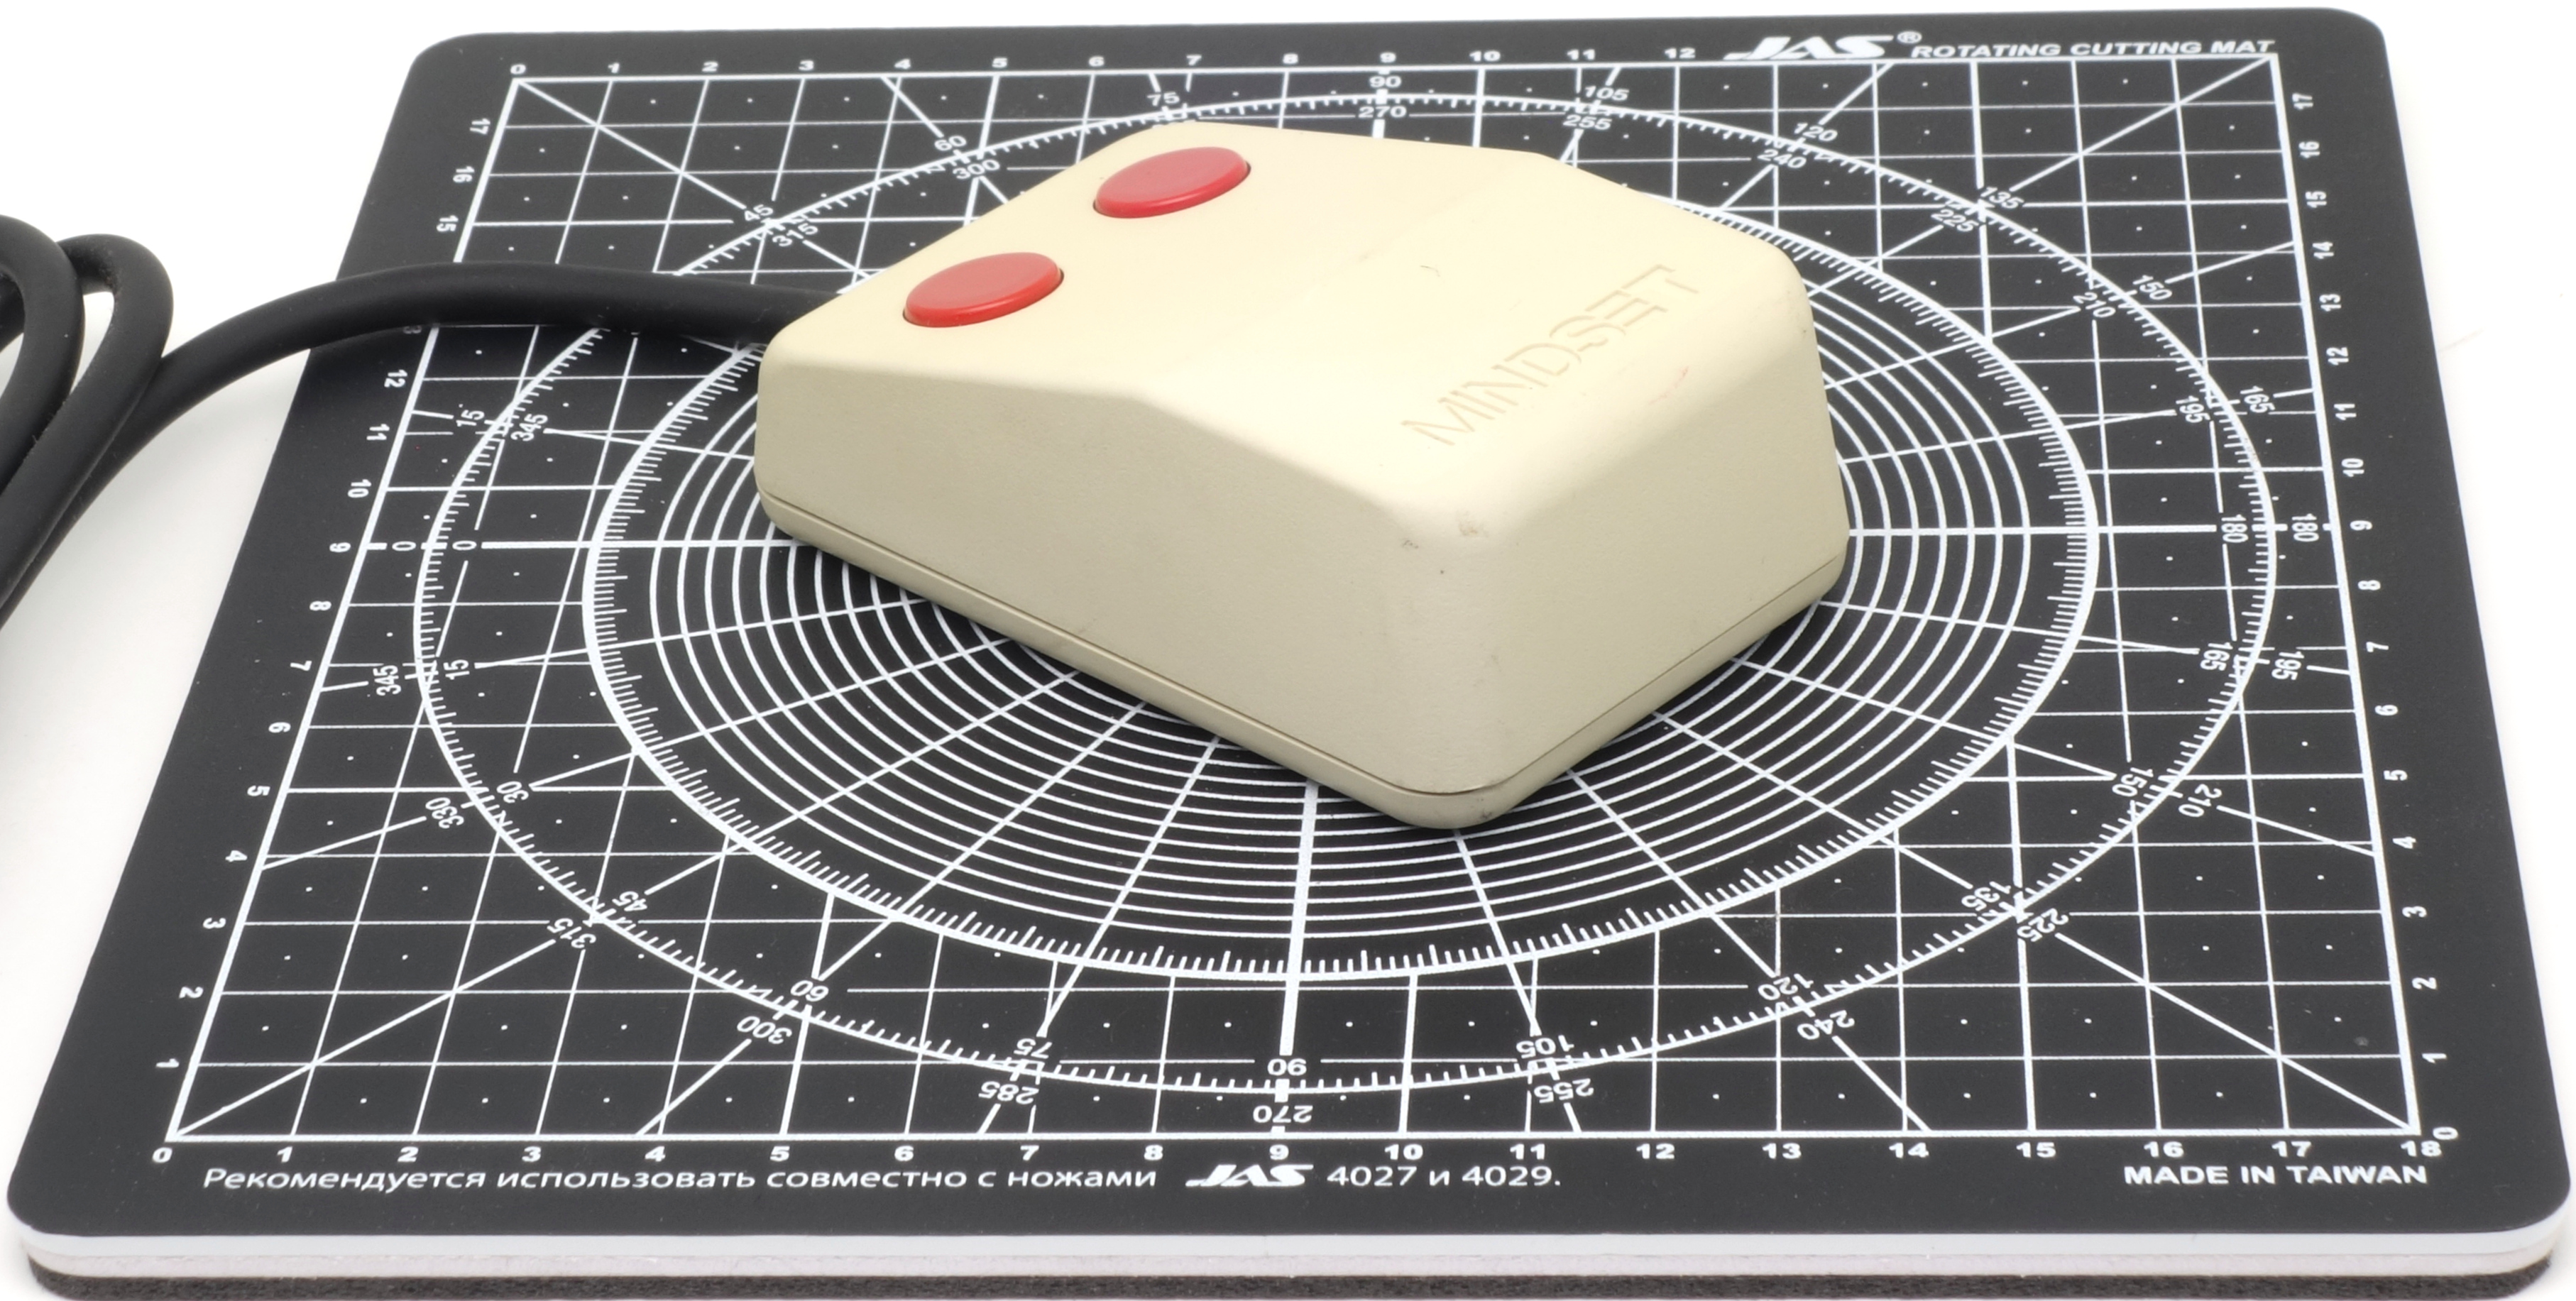
\includegraphics[scale=0.5]{1984_mindset_mouse/size_15.jpg}
    \caption{Mindset Mouse на размерном коврике с шагом сетки 1~см}
    \label{fig:MindsetMouseSize}
\end{figure}

И без того небольшой размер мыши (рис. \ref{fig:MindsetMouseSize}) кажется еще меньшим за счет клиновидной формы (наклонная часть занимает две трети длины корпуса), однако при этом мышь довольно тяжелая. Стремление разработчиков добиться яркого дизайна сказалось на эргономике не самым лучшим образом. Кнопки имеют малый размер и не самое идеальное расположение (они находятся на некотором удалении от края корпуса, что сказывается на особенностях захвата мыши ладонью). Ближняя к пользователю грань корпуса практически вертикальна, однако даже будь она наклонной, с учетом размеров мыши существенных улучшений в эргономику это не внесло бы (рис. \ref{fig:SharpMZ1x10Hand}).

\begin{figure}[h]
    \centering
    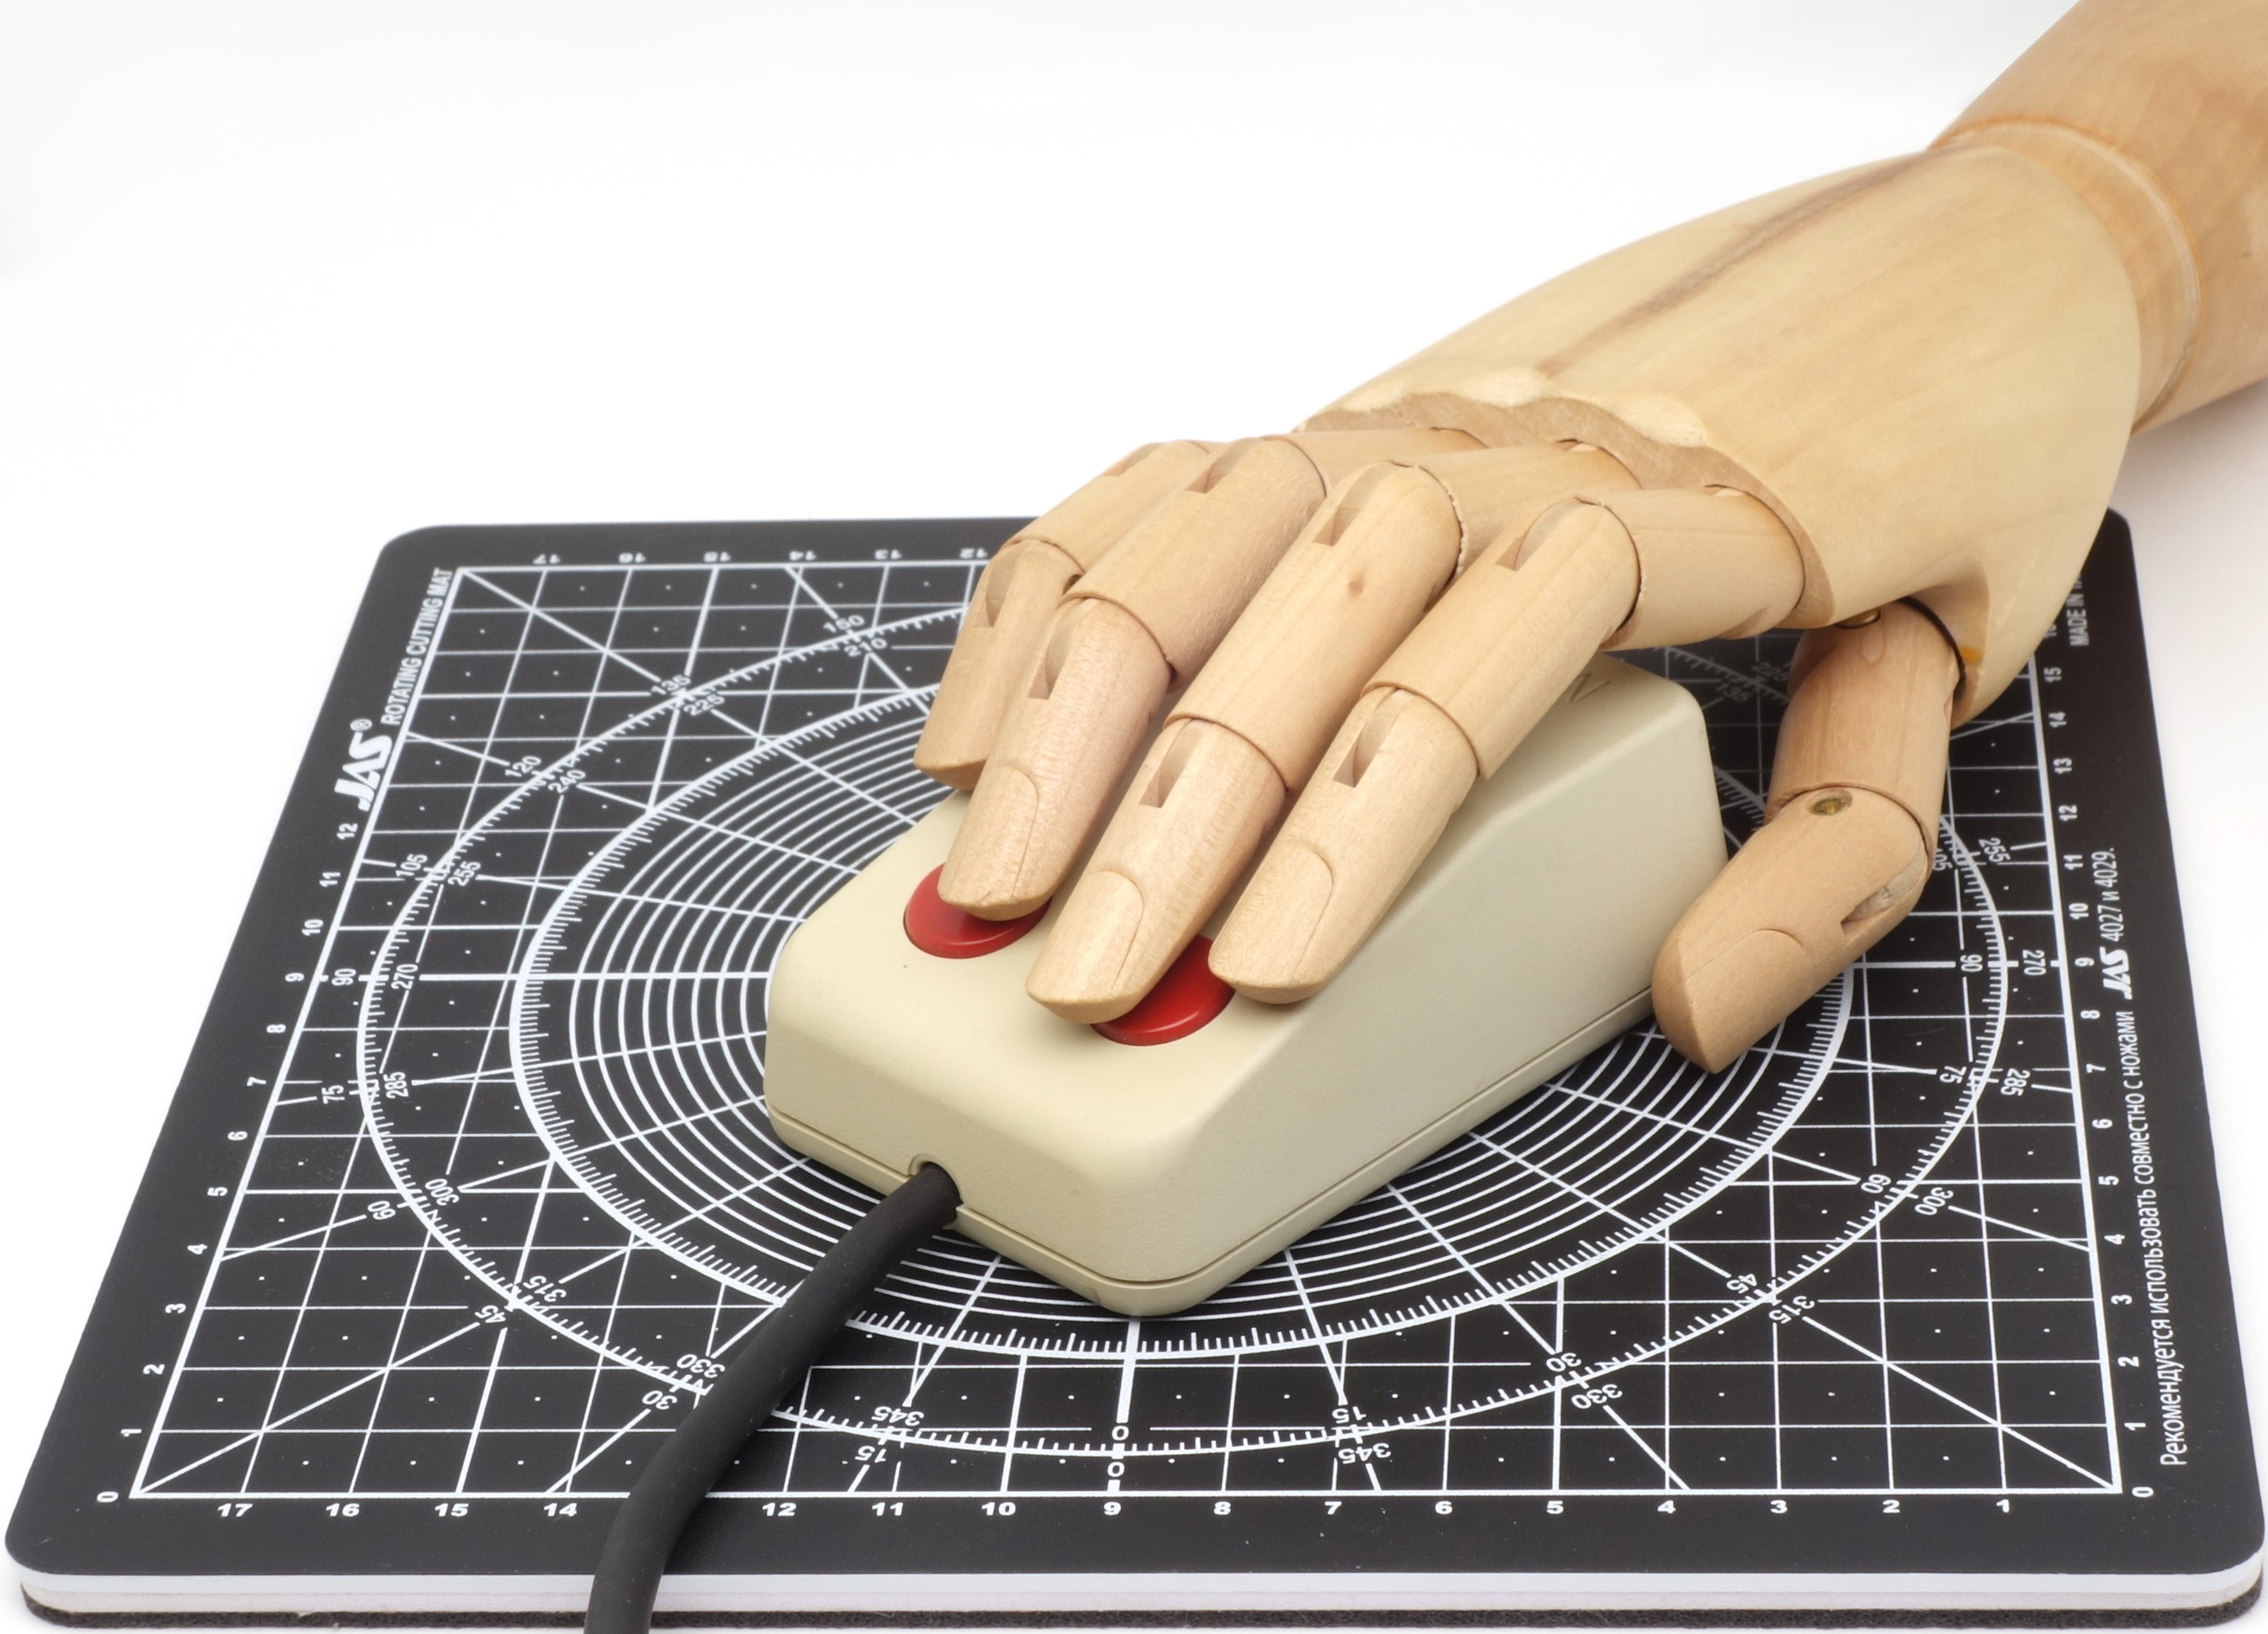
\includegraphics[scale=0.5]{1984_mindset_mouse/hand_30.jpg}
    \caption{Mindset Mouse с моделью руки человека}
    \label{fig:MindsetMouseHand}
\end{figure}

Внутреннее устройство мыши показано на рис. \ref{fig:MindsetMouseInside}. В мыши использована конструкция мышей Alps первого поколения на базе закрытых контактных энкодеров. При сравнении с другими изделиями на базе этой конструкции "--- мышью MZ-1X10 и первой мышью компании Microsoft "--- обнаруживается почти полная идентичность конструкции, за исключением конфигурации печатных плат и элементов, свзяанных с разными интерфейсами подключения мыши.

 \begin{figure}[h]
    \centering
    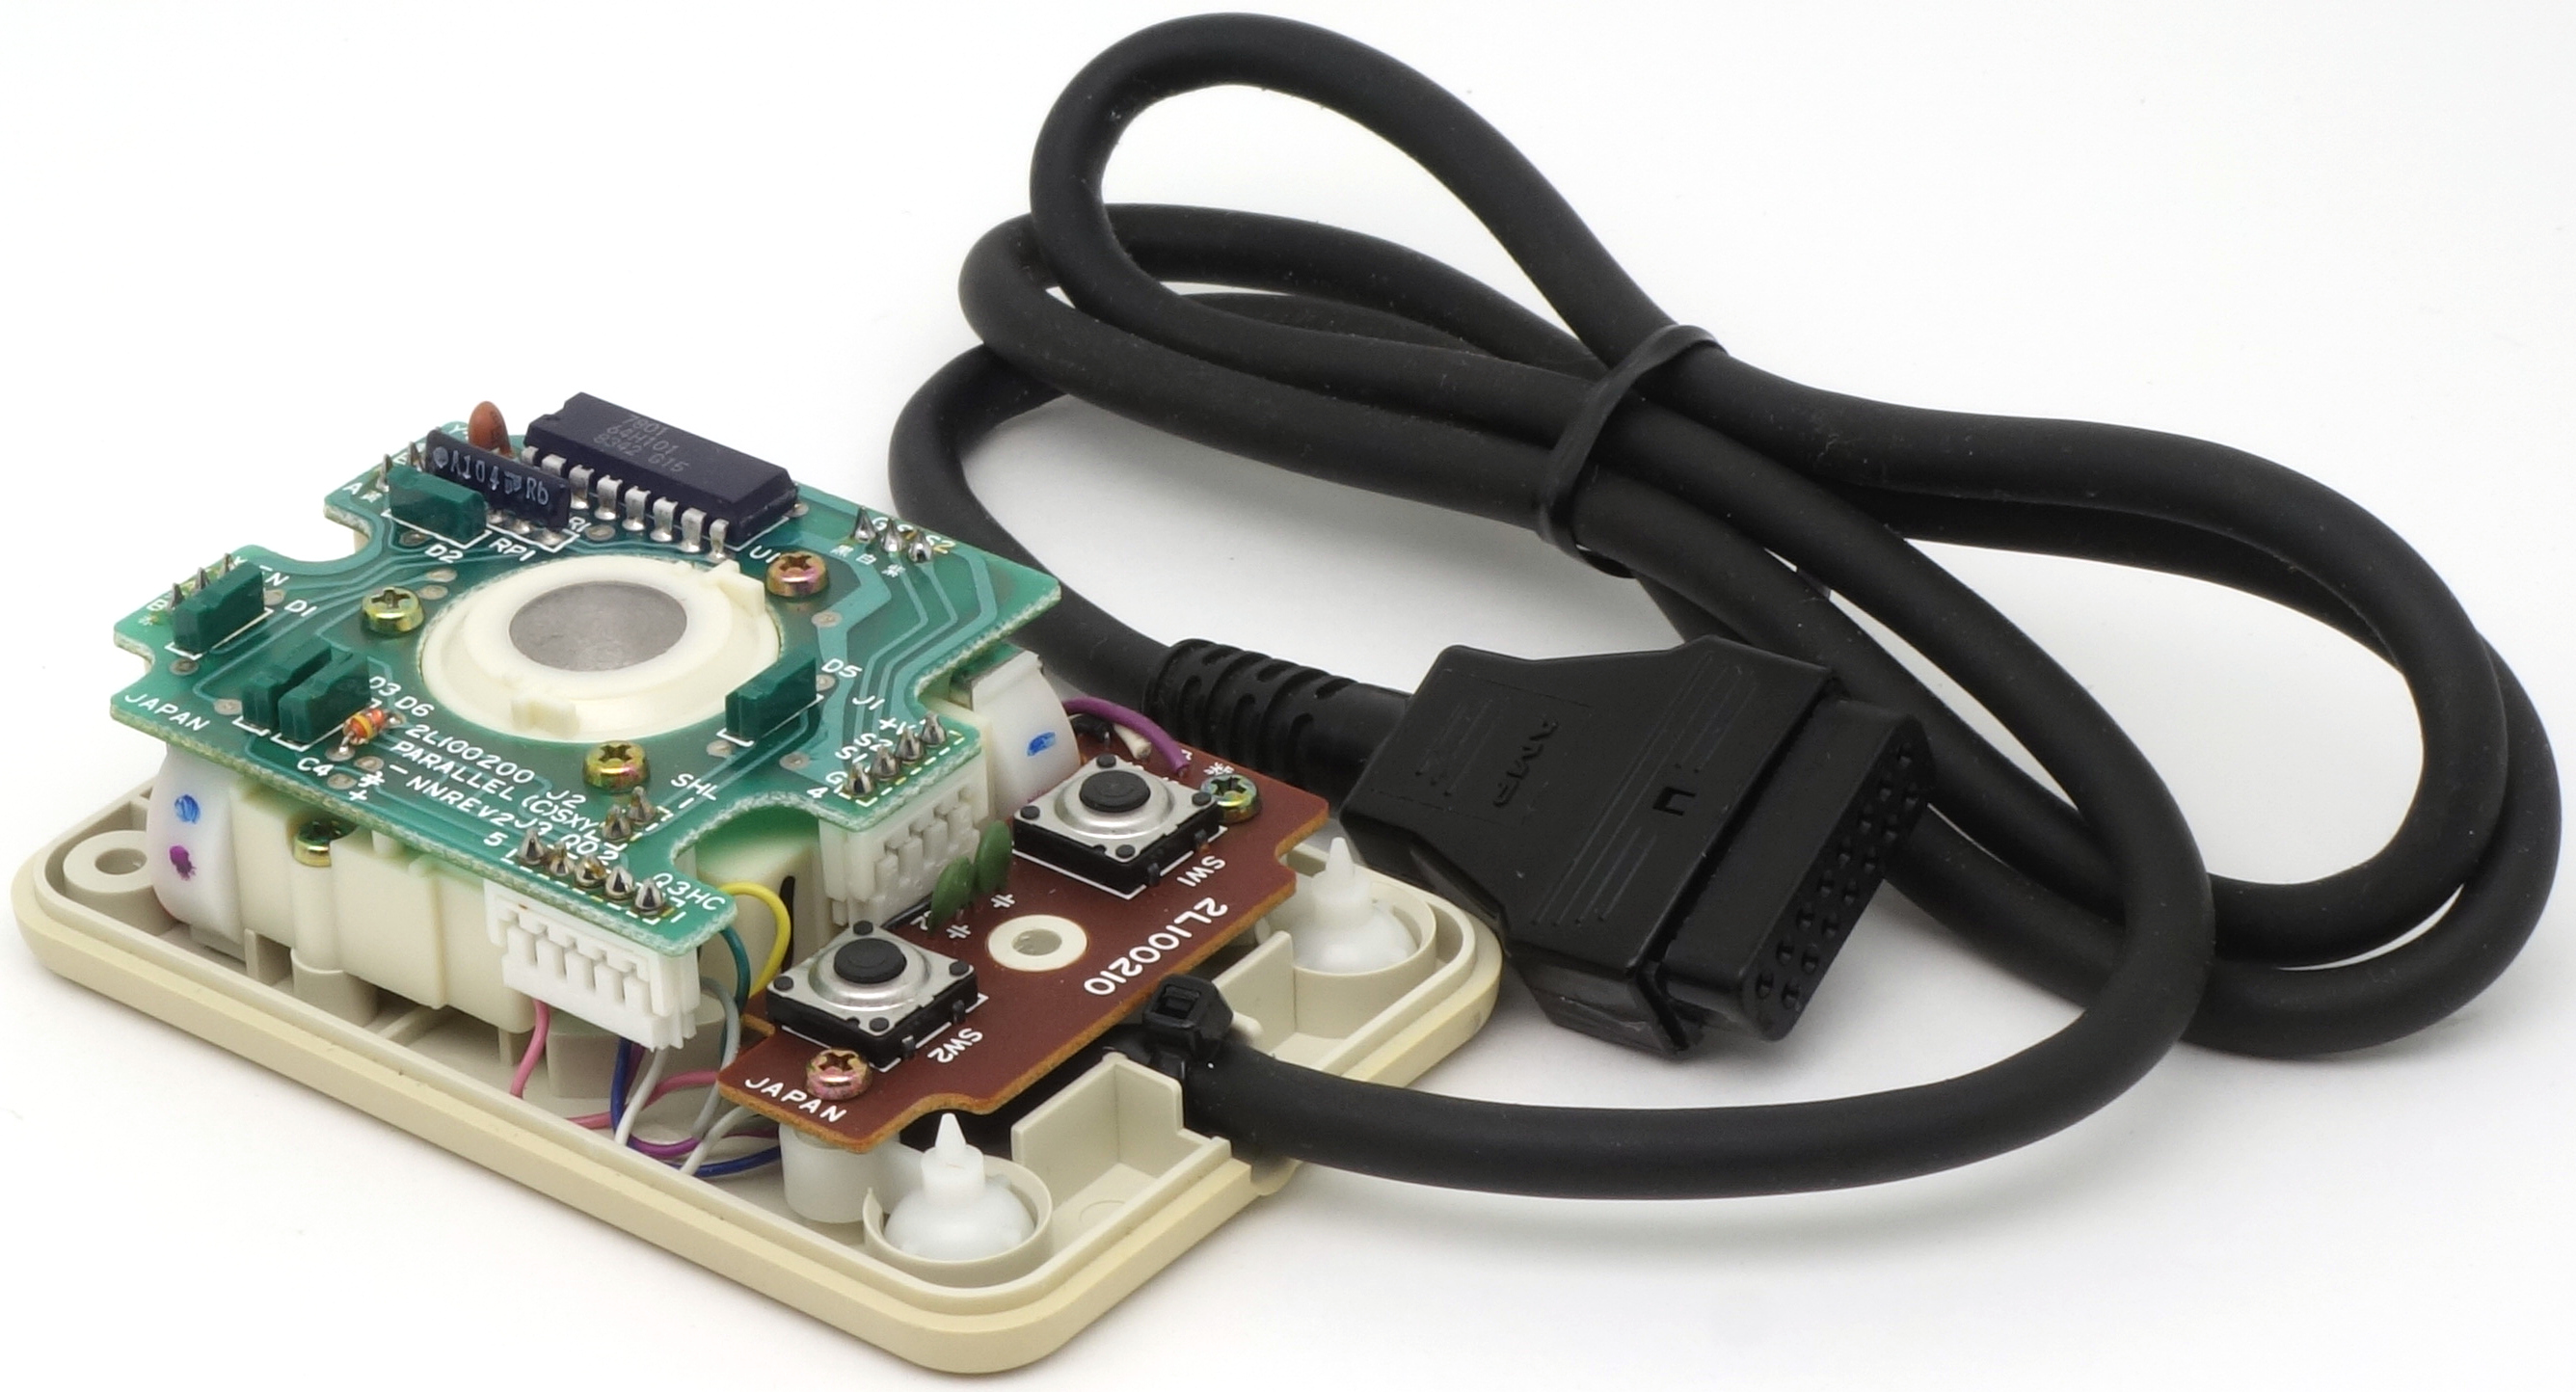
\includegraphics[scale=1]{1984_mindset_mouse/inside_30.jpg}
    \caption{Mindset Mouse в разобранном виде}
    \label{fig:MindsetMouseInside}
\end{figure}



\begin{thebibliography}{9}
\bibitem {byteMagazine} Wadlow T. The Mindset Personal Computer // Byte Magazine, Vol. 10, No. 6. June, 1985. - P. 324-232 \url{https://archive.org/details/byte-magazine-1985-06/page/n331/mode/2up}
\bibitem{adv} Mindset Personal Computer System \url{https://archive.org/details/bitsavers_mindsetBrore_3744143/page/n1/mode/2up?q=%22mindset+mouse%22}
\end{thebibliography}
\end{document}
